\chapter{}

\titleimg{hail}

\mktitle{Capitulum Duodecimum}
\thispagestyle{empty}

\vnum{1}Dīxit quoque Dominus ad Moysēn et Aarōn in terrā
Ægyptī: \vnum{2}``Mēnsis iste, vōbīs prīncipium mēnsium: prīmus erit in mēnsibus
annī. \vnum{3}Loquiminī ad ūniversum cœtum fīliōrum Isrāēl, et
dīcite eīs: Decima diē mēnsis huius tollat ūnusquisque agnum per familiās
et domōs suās. \vnum{4}Sīn autem minor est numerus ut \mpp{sufficere:}{satis esse}sufficere
possit ad \mpp{vēscī:}{ēdere}vēscendum agnum, assūmet \mpp{vicinus/a/um:}{prope habitans}vīcīnum suum quī iūnctus est domuī suæ, iuxtā numerum
animārum quæ sufficere possunt ad ēsum agnī.''

\vnum{5}``Erit autem agnus absque
\mpp{macula, -ae (f):}{pars in quā proprius color abest}maculā,
\mpp{masculus/a/um:}{masculīnus}masculus, \mpp{anniculus/a/um:}{unius annī}anniculus:
iuxtā quem \mpp{rītus, -ūs (m):}{res agendae ut sacra recte fiant}rītum
tollētis et \mimg{babygoat}{haedus, -ī (m)}hædum. \vnum{6}Et
servābitis eum usque ad quartamdecimam diem mēnsis huius:
\mpp{immolare:}{sacrificium facere}immolābitque eum ūniversa multitūdō
fīliōrum Isrāēl ad \mpp{vespera, -ae (f) =}{vesper}vesperam.''

\begin{figure}[h!]
    \begin{minipage}[hp]{0.5\linewidth}
        \centering
        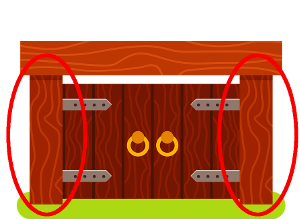
\includegraphics{postis}
        \caption{postis, -is (m)}
    \end{minipage}%
    \begin{minipage}[hp]{0.5\linewidth}
        \centering
        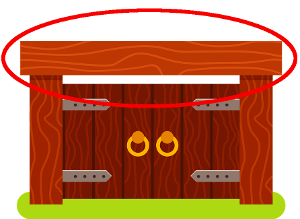
\includegraphics{superlimen}
        \caption{superlīmināre, -is (n)}
    \end{minipage}
\end{figure}

\vnum{7}``Et sūment dē sanguine eius,
ac pōnent super utrumque postem, et in
superlīmināribus \mimg{lactuca}{lactūca, -ae (f)}domōrum, in quibus \mpp{comedere:}{totum
esse; esse}comedent illum. \vnum{8}Et edent carnēs nocte illa
\mpp{assus/a/um}{sine aquā vel aliā materiā fluentī coctus}assās ignī, et
\mpp{azȳmus/a/um:}{sine materiā quae efficit ut panis turgidus fiat}azȳmōs pānēs cum lactūcīs \mpp{agrestis, -e (adj):}{ad agros pertinens; rudis}agrestibus. \vnum{9}Nōn
comedētis ex eō \mpp{crūdus/a/um:}{non coctus}crūdum quid, nec coctum aquā, sed tantum
assum ignī: caput cum pedibus eius et intestīnīs
vorābitis.''

\begin{figure}[h!]
    \begin{minipage}[hp]{0.5\linewidth}
        \centering
        
\includegraphics{intestine}
        \caption{intestīnus, -ī (m)}
    \end{minipage}%
    \begin{minipage}[hp]{0.5\linewidth}
        \centering
        
\includegraphics{renes}
        \caption{rēnēs, rēnum (m)}
    \end{minipage}
\end{figure}

\vnum{10}``Nec remanēbit quidquam ex eō usque manē; sī quid
\mpp{residuus:}{quod reliquum est}residuum fuerit, igne
\mpp{comburere:}{igne perdere}combūrētis. \vnum{11}Sīc autem comedētis illum:
\mpp{rēnēs accingere:}{induere vestis quae cingit corpus circiter rēnēs}rēnēs vestrōs \mpp{accingere =}{cingere}accingētis, et
\mpp{calceamentum:}{quod pedi induitur}calceāmenta habēbitis in pedibus,
tenentēs baculōs in manibus, et comedētis \mpp{festīnanter =}{celeriter}festīnanter: est
enim \mpp{Phase:}{vocabulum Hebraicum}Phase (id est, trānsitus) Dominī. \vnum{12}Et trānsībō per
terram Ægyptī nocte illa, percutiamque omne \mpp{????}{????}prīmōgenitum in
terrā Ægyptī ab homine usque ad pecūs: et in cūnctīs dīīs Ægyptī faciam
\mpp{????}{????}iūdicia. Ego Dominus. \vnum{13}Erit autem sanguis vōbīs in signum
in \mpp{????}{????}ædibus in quibus eritis: et vidēbō sanguinem, et
trānsībō vōs: nec erit in vōbīs \mpp{plaga:}{e.g, unus pulsat alterum eo
tempore cum pugnus corpus tangit `plaga' vocatur}plāgā
\mpp{????}{????}disperdēns quandō percusserō terram Ægyptī. \vnum{14}Habēbitis
autem hunc diem in \mpp{????}{????}monumentum: et
\mpp{????}{????}celebrābitis eam \mpp{????}{????}sōlemnem Dominō in
\mpp{????}{????}generātiōnibus vestrīs cultū \mpp{????}{????}sempiternō.
\vnum{15}Septem diēbus azȳma comedētis: in diē prīmō nōn erit
\mpp{????}{????}fermentum in domibus vestrīs: quīcumque comēderit
\mpp{????}{????}fermentātum, perībit anima illa dē Isrāēl, ā prīmō diē
usque ad diem septimum. \vnum{16}Diēs prīma erit \mpp{????}{????}sānctā atque
\mpp{????}{????}sōlemnis, et diēs septima eādem \mpp{????}{????}fēstīvitāte
\mpp{????}{????}venerābilis: nihil operis faciētis in eīs,
\mpp{????}{????}exceptīs hīs, quæ ad vēscendum \mpp{pertinere:}{e.g,
colloquium ad me pertinet si homines loquuntur de me}pertinent. \vnum{17}Et
\mpp{????}{????}observābitis azȳma: in eādem enim ipsā diē ēdūcam
exercitum vestrum dē terrā Ægyptī, et cūstōdiētis diem istum in
\mpp{????}{????}generātiōnēs vestrās \mpp{????}{????}rītū perpetuō.
\vnum{18} Prīmō mēnse, \mpp{????}{????}quartadecīmā diē mēnsis ad vesperam, comedētis
azȳma usque ad diem \mpp{????}{????}vīgēsimam prīmam eiusdem mēnsis ad
vesperam. \vnum{19}Septem diēbus fermentum nōn inveniētur in domibus vestrīs:
quī comēderit fermentātum, perībit anima eius dē cœtū Isrāēl, tam dē
advenīs quam dē \mpp{????}{????}indigenīs terræ. \vnum{20}Omne fermentātum nōn
comedētis: in cūnctīs \mpp{????}{????}habitāculīs vestrīs edētis azȳma.''

\vnum{21}Vocāvit autem Moysēs omnēs seniōrēs fīliōrum Isrāēl, et
dīxit ad eōs: ``Īte tollentēs animal per familiās vestrās, et immolātē
Phase. \vnum{22}\mpp{????}{????}Fasciculumque \mpp{????}{????}hyssōpī
\mpp{????}{????}tingite in sanguine quī est in līmine, et aspergite ex eō
\mpp{????}{????}superlīmināre, et utrumque postem: nūllus vestrum
ēgrediātur ōstium domūs suæ usque manē. \vnum{23}Trānsībit enim Dominus
percutiēns Ægyptiōs: cumque vīderit sanguinem in
superlīminārī, et in utrōque poste,
\mpp{????}{????}trānscendet ōstium domūs, et nōn sinet
\mpp{????}{????}percussōrem \mpp{ingredi:}{intus ire}ingredī domōs vestrās
et lædere. \vnum{24}Cūstōdī verbum istud \mpp{????}{????}lēgitimum tibi et fīliīs
tuīs usque in \mpp{????}{????}æternum. \vnum{25}Cumque \mpp{introire:}{intus ire;
ingredi}introierītis terram, quam Dominus datūrus est vōbīs ut pollicitus
est, observābitis \mpp{????}{????}cæremōniās istās. \vnum{26}Et cum dīxerint
vōbīs fīliī vestrī: Quæ est ista \mpp{????}{????}religiō? \vnum{27}Dīcētis eīs:
\mpp{????}{????}Victima trānsitūs Dominī est, quandō trānsīvit super
domōs fīliōrum Isrāēl in Ægyptō, percutiēns Ægyptiōs, et domōs nostrās
līberāns.''

\mpp{????}{????}Incurvātusque populus adōrāvit. \vnum{28}Et ēgressī
fīliī Isrāēl fēcērunt sīcut \mpp{praecipere:}{imperare}præcēperat Dominus
Moȳsī et Aarōn. \vnum{29}Factum est autem in noctīs mediō, percussit Dominus omne
prīmōgenitum in terrā Ægyptī, ā \mpp{????}{????}prīmōgenitō
Pharaōnis, quī in soliō eius sedēbat, usque ad prīmōgenitum
\mpp{????}{????}captīvæ quæ erat in carcere, et omne prīmōgenitum
\mpp{iumentum:}{animal utile ad gerendum vel trahendum e.g, equi, boves, et
cetera}iūmentōrum. \vnum{30}Surrēxitque Pharaō nocte, et omnēs
servī eius, cūnctaque Ægyptus: et ortus est clāmor magnus in Ægyptō:
neque enim erat domus in quā nōn iacēret mortuus. \vnum{31}Vocātīsque Pharaō
Moyse et Aarōn nocte, ait: Surgite et ēgrediminī ā populō
meō, vōs et fīliī Isrāēl: īte, immolātē Dominō sīcut dīcitis. \vnum{32}Ovēs
vestrās et \mpp{????}{????}armenta assūmite ut petierātis, et abeuntēs
\mpp{????}{????}benedīcite mihi. \vnum{33}\mpp{????}{????}Urgēbantque Ægyptiī
populum dē terrā exīre vēlōciter, dīcentēs: Omnēs moriēmur. \vnum{34}Tulit
igitur populus \mpp{????}{????}cōnspersam \mpp{????}{????}farīnam antequam
\mpp{????}{????}fermentārētur: et ligāns in palliīs, posuit super
\mpp{????}{????}humerōs suōs. \vnum{35}Fēcēruntque fīliī Isrāēl sīcut præcēperat
Moysēs: et petiērunt ab Ægyptiīs vāsa argentea et aurea, vestemque
plūrimam. \vnum{36}Dominus autem dedit grātiam populō cōram Ægyptiīs ut
\mpp{????}{????}commodārent eīs: et \mpp{spoliare:}{capere res aliorum
hominum}spoliāvērunt Ægyptiōs. \vnum{37}Profectīque sunt fīliī Isrāēl dē Ramesse
in Socoth, sexcenta ferē mīllia peditum virōrum, absque parvulīs. \vnum{38}Sed et
\mpp{????}{????}vulgus \mpp{????}{????}prōmiscuum \mpp{innumerabilis:}{qui
numerari non potest}innumerābile ascendit cum eīs, ovēs et armenta et
animantia \mpp{diversus:}{in varias partes versi sunt}dīversī generis multa
nimis. \vnum{39}Coxēruntque farīnam, quam \mpp{????}{????}dūdum dē Ægyptō
cōnspersam tulerant: et fēcērunt \mpp{????}{????}subcinerīciōs pānēs
azȳmōs: neque enim poterant \mpp{????}{????}fermentārī, cōgentibus exīre
Ægyptiīs, et nūllam facere sinentibus moram: nec \mpp{????}{????}pulmentī
quidquam occurrerat \mpp{????}{????}præparāre. \vnum{40}\mpp{????}{????}Habitātiō
autem fīliōrum Isrāēl quā mānsērunt in Ægyptō, fuit quadringentōrum
trīgintā annōrum. \vnum{41}Quibus \mpp{explere:}{perficere}explētis, eādem diē
ēgressus est omnis exercitus Dominī dē terrā Ægyptī. \vnum{42}Nox ista est
observābilis Dominī, quandō ēdūxit eōs dē terrā Ægyptī: hanc
\mpp{????}{????}observāre dēbent omnēs fīliī Isrāēl in generātiōnibus suīs.
\vnum{43}Dīxitque Dominus ad Moysēn et Aarōn: Hæc est religiō Phase: omnis
\mpp{????}{????}aliēnigena nōn comedet ex eō. \vnum{44}Omnīs autem servus
emptitius \mpp{????}{????}circumcīdētur, et sīc comedet. \vnum{45}Advena et
\mpp{????}{????}mercēnārius nōn edent ex eō. \vnum{46}In ūnā domō comedētur, nec
\mpp{????}{????}efferētis dē carnibus eius forās, nec os illīus
\mpp{confringere:}{una frangere}cōnfringētis. \vnum{47}Omnīs cœtūs fīliōrum
Isrāēl faciet illud. \vnum{48}Quod sī quis \mpp{????}{????}peregrīnōrum in
vestram voluerit trānsīre \mpp{????}{????}colōniam, et facere Phase Dominī,
circumcīdētur prius omne masculīnum eius, et tunc \mpp{????}{????}rīte
\mpp{????}{????}celebrābit: eritque sīcut \mpp{????}{????}indigena terræ:
sī quis autem \mpp{????}{????}circumcīsus nōn fuerit, nōn
\mpp{????}{????}vēscētur ex eō. \vnum{49}Eādem lēx erit \mpp{????}{????}indigenæ
et colōnō quī \mpp{????}{????}peregrīnātur apud vōs. \vnum{50}Fēcēruntque omnēs
fīliī Isrāēl sīcut præcēperat Dominus Moȳsī et Aarōn. \vnum{51}Et eādem diē
ēdūxit Dominus fīliōs Isrāēl dē terrā Ægyptī per \mpp{????}{????}turmās
suās. 
